\section{Methods}

\subsection{The experts}
The experts are 6 fellow CSE undergraduate students, who are independently working on a different implementation of TALIO. They have the same application in mind and know the ins and outs of what the functionalities should be. Yet they have a different outlook on how a user should experience the talio application, and thus how well our design for talio is made with the user in mind. 

\subsection{The visuals}
 The experts were sent a link to a Google Docs document. Each page of this document shows a specific part of our design. So one page shows how one can add a list, another shows how to edit a card, et cetera. We show this by screenshots and digital drawings of the interface. Sometimes, a feature was hard to demonstrate with a static image, e.g. the ability to drag and drop cards. In these cases, we added a little text to clarify. In addition, we described what each button on a certain page does and added a hyperlink to the relevant page in our prototype. This allowed the experts to actually explore the interface.

See \ref{fig:ExamplePrototypeAddCard} for one example of such a page. This page shows the design made in paint.NET. The screenshot shows the interface to add a card. This is overlaid on top of the interface of the board to make it clear it is a pop-up. Below the image, you can see the text with hyperlinks so that users of the prototype can easily navigate through it.
\begin{figure}
    \centering
    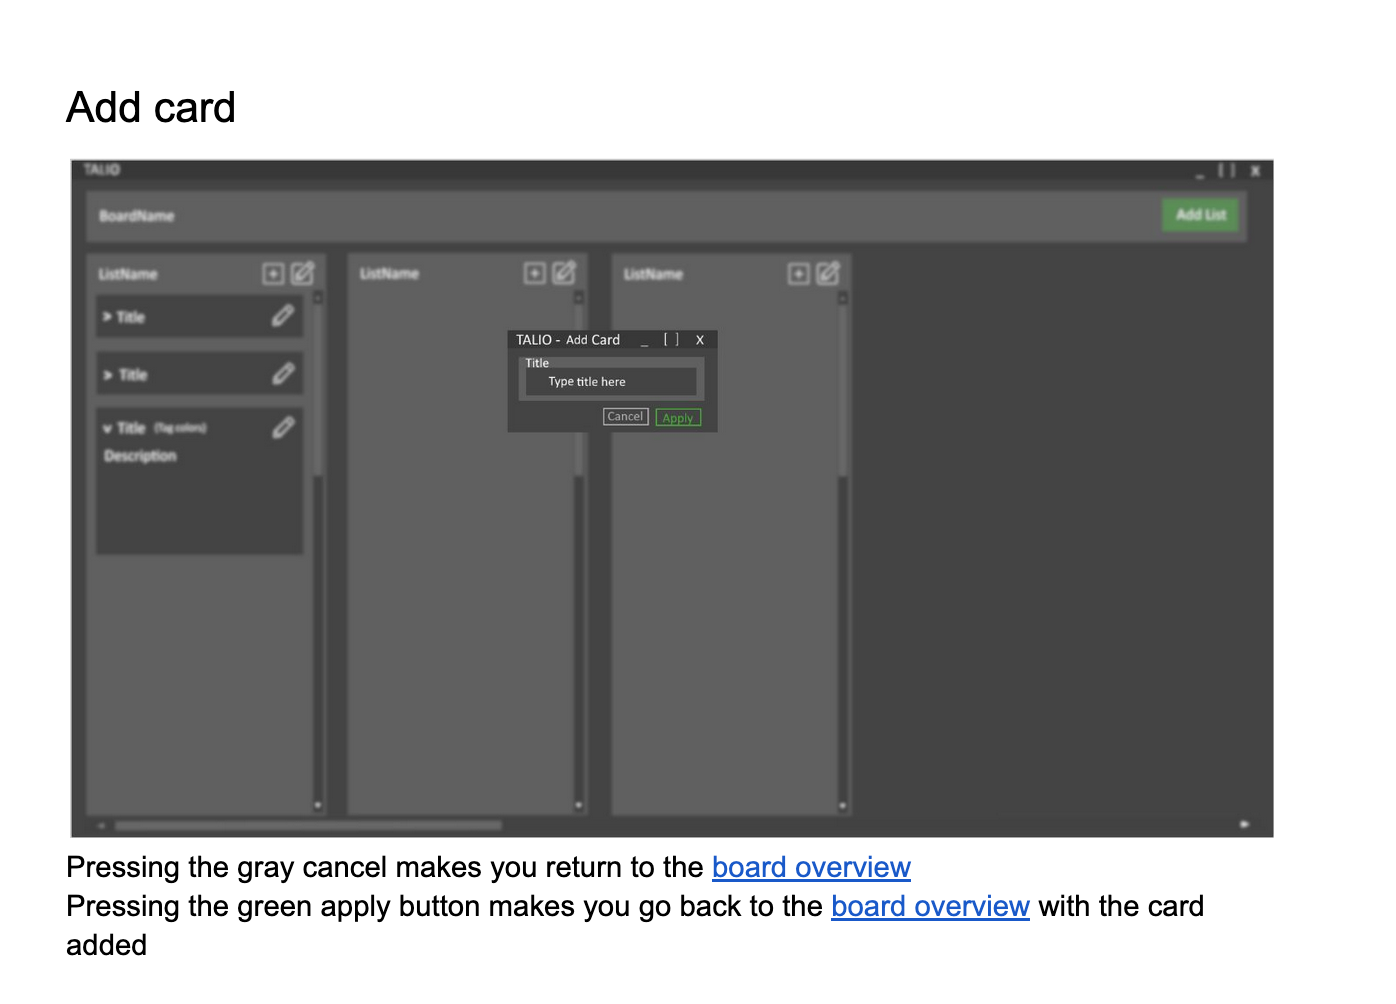
\includegraphics[width=\linewidth]{images/ExamplePrototypeAddCard.png}
    \caption{One of the pages in our prototype. This page shows the interface for adding a card.}
    \label{fig:ExamplePrototypeAddCard}
\end{figure}

Another example is \ref{fig:ExamplePrototypeConnect}. This time the page has a screenshot of our current implementation. This is the page for connecting to the server.


\begin{figure}
    \centering
    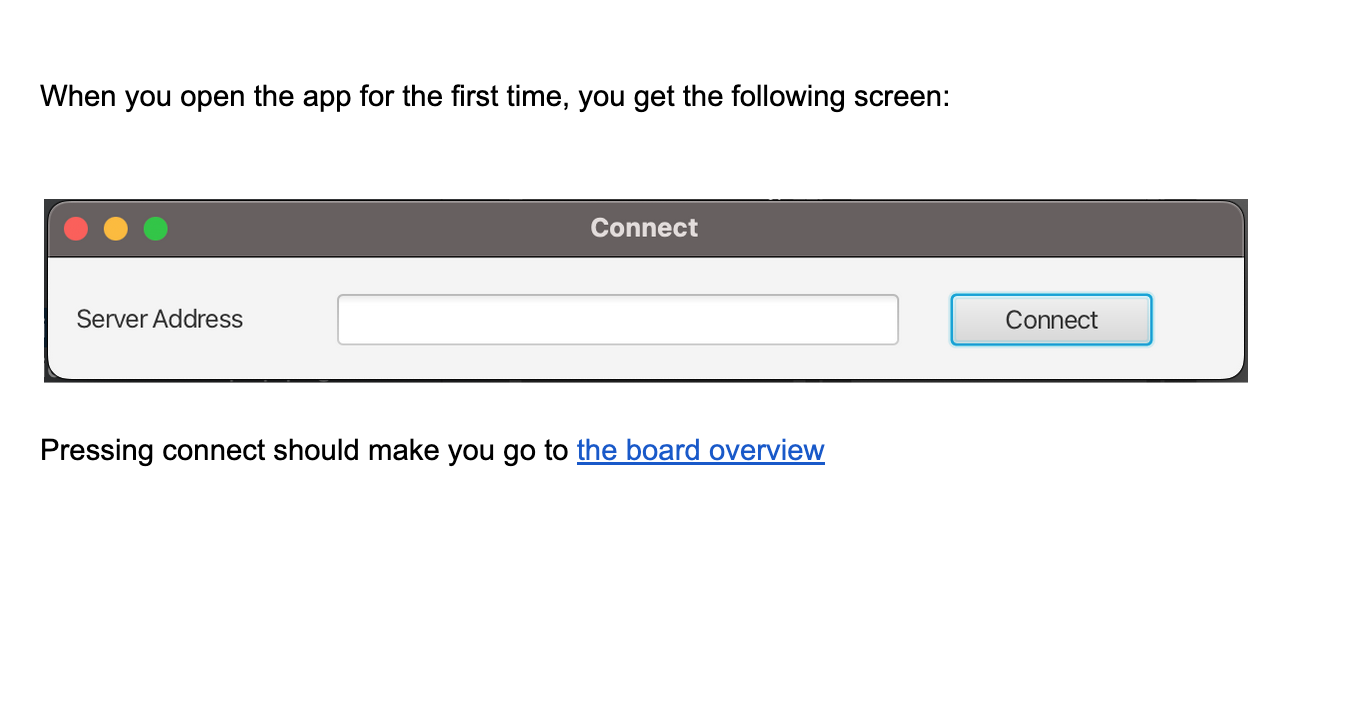
\includegraphics[width=\linewidth]{images/ExamplePrototypeConnect.png}
    \caption{Another page of our prototype. This page shows the interface for connecting to the server.}
    \label{fig:ExamplePrototypeConnect}
\end{figure}

\subsection{The task of the experts}
The experts needed to evaluate the prototype sent to them using 10 heuristics. The experts were asked to first explore our prototype. Then they were supposed to look at every page and, keeping the heuristics (see next section) in mind think about what could go wrong. In the end, they should have a list of problems they encountered.

\subsection{The heuristics}
The experts were asked to consider the following ten heuristics:
\begin{enumerate}
\item Visibility of system status:
The user should always be able to see what's going on. Multi-step processes make it clear in which step you are.\cite{video-slides}

\item Match between system and the real world
Words familiar to the user should be used. Don't introduce unnecessary jargon that the user would have to learn.\cite{video-slides}

\item User control and freedom:
If a user makes a mistake, it should be easily reversible.\cite{video-slides}

\item Consistency and standards:
If two things do the same thing, they should also look the same. Don't confuse the user with non-existing differences.\cite{video-slides}

\item Error prevention:
Make sure as little errors can occur as possible. Design the UI such that users are unlikely to accidentally cause errors.\cite{video-slides}

\item Recognition rather than recall:
Display all the data and actions a user can perform. Make it so that the user won't have to remember a lot of stuff do perform a basic action.\cite{video-slides}

\item Flexibility and efficiency of use:
Give shortcuts to the user and allow them to customize it so that they can perform a tasks faster. Give power users the tools they want.\cite{video-slides}

\item Aesthetic and minimalist design:
Don't overload the user with unnecessary data. Only show what's necessary for them to perform what they want to do.\cite{video-slides}

\item Help users recognize, diagnose, and recover from errors:
Users should be able to understand error messages. When they get an error message, they should know how to solve the problem. \cite{video-slides}

\item Help and documentation:
Provide the user with explanation of what they can do and how to do something. Allow them to easily access documentation relevant to their current options. 
\cite{video-slides}
\end{enumerate}
\hfill \break
These heuristics come from Nielsen, 1994\cite{nielsen1994heuristic}.

\subsection{Measurements}
We are measuring our TALIO application against the heuristics. The experts should give a detailed evaluation containing a list of problems, each with a description, scene, and corresponding heuristic. A problem is defined as something that is a missing feature, according to the user stories, or something which does not align with any of the heuristics. A description should describe what the problem is, and the scene should describe when this problem occurs. 

